\documentclass{standalone}
\usepackage{mintikz}

\begin{document}
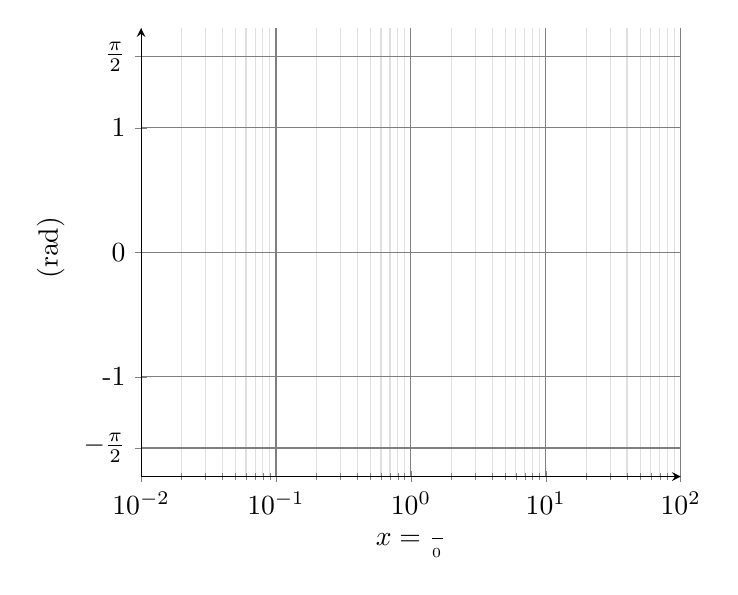
\begin{tikzpicture}[]
	\begin{semilogxaxis}[
			xmin=1e-2, xmax=1e2,
			ymin=-1.8, ymax=1.8,
			xlabel={$x=\DS\frac{\w}{\w_0}$}, ylabel=$\f$ (rad),
			ytick={-1.57079, -1, 0, 1, 1.57079},
			yticklabels={$\DS-\frac{\pi}{2}$, -1, 0, 1, $\DS\frac{\pi}{2}$},
			% extra y ticks={0.78539, 1.57079},
			% extra y tick labels={$\DS\frac{\pi}{4}$, $\DS\frac{\pi}{2}$},
			% extra y tick style={grid=none},
			axis lines=left,
			grid=both,
			major grid style={black!50},
			minor grid style={gray!25},
			clip=true]
		\def\Q{5}
		% \addplot[
		% domain=1e-2:1e2, samples=500,
		% smooth, thick, red]
		% {-atan(\Q*(\x-1/\x))*pi/180};
		% \def\Q{.5}
		% \addplot[
		% domain=1e-2:1e2, samples=500,
		% smooth, thick, blue]
		% {-atan(\Q*(\x-1/\x))*pi/180};
		% \addplot[
		% domain=1e-2:2,
		% smooth, black, dashed, thick]
		% {pi/2};
		% \addplot[
		% domain=6e-1:1e2,
		% smooth, black, dashed, thick]
		% {-pi/2};
		% \node[red] at (axis cs:2.5,.8) {$Q=5$};
		% \node[blue] at (axis cs:.2,.5) {$Q=0.5$};
		% \draw[dashed, thick]
		% (axis cs:1e-2,0) -|
		% (axis cs:1e0,-1.8);
	\end{semilogxaxis}
\end{tikzpicture}
\end{document}
